\section{Testing}
\label{sec:testing}
In this section we show the testing application we have developed to assess the functionalities of the implemented classes described in \S\ref{sec:implementation}.

\subsection{A sample application}
In \hyperref[fig:sample-app]{\textbf{Figure \ref{fig:sample-app}}} we show a sample application developed to test the implemented classes for communication. As it can be seen, the structure of the application is very simple, we have three groups communicating in a pipeline fashion, by means of implemented \texttt{sender} and \texttt{receiver} nodes. Communication between groups can happen with the different plugins provided by the Mercury library, and switching from one plugin (transport) to another is only a matter of passing as configuration string the desired plugin (transport) to use for communication.\newline

\hr{fig:node-legends}{Figure} shows the legend for the nodes and communication channels used in the sample application. We have two types of nodes, sequential ones which are standard \ttt{ff\_node\_t}, and Margo-injected nodes which are used for communication between distributed groups. Simple plain arrows indicates usual FastFlow shared memory channel, instead bullet-tailed arrows indicate a distributed connection between two nodes. Note, however, that ``distributed'' here only means that two groups are connected through Margo calls, but the nodes can reside in the same machine and communicate with the shared memory plugin provided by Margo, as it happened in part of the testing phase.

\begin{figure}[H]
    \centering
    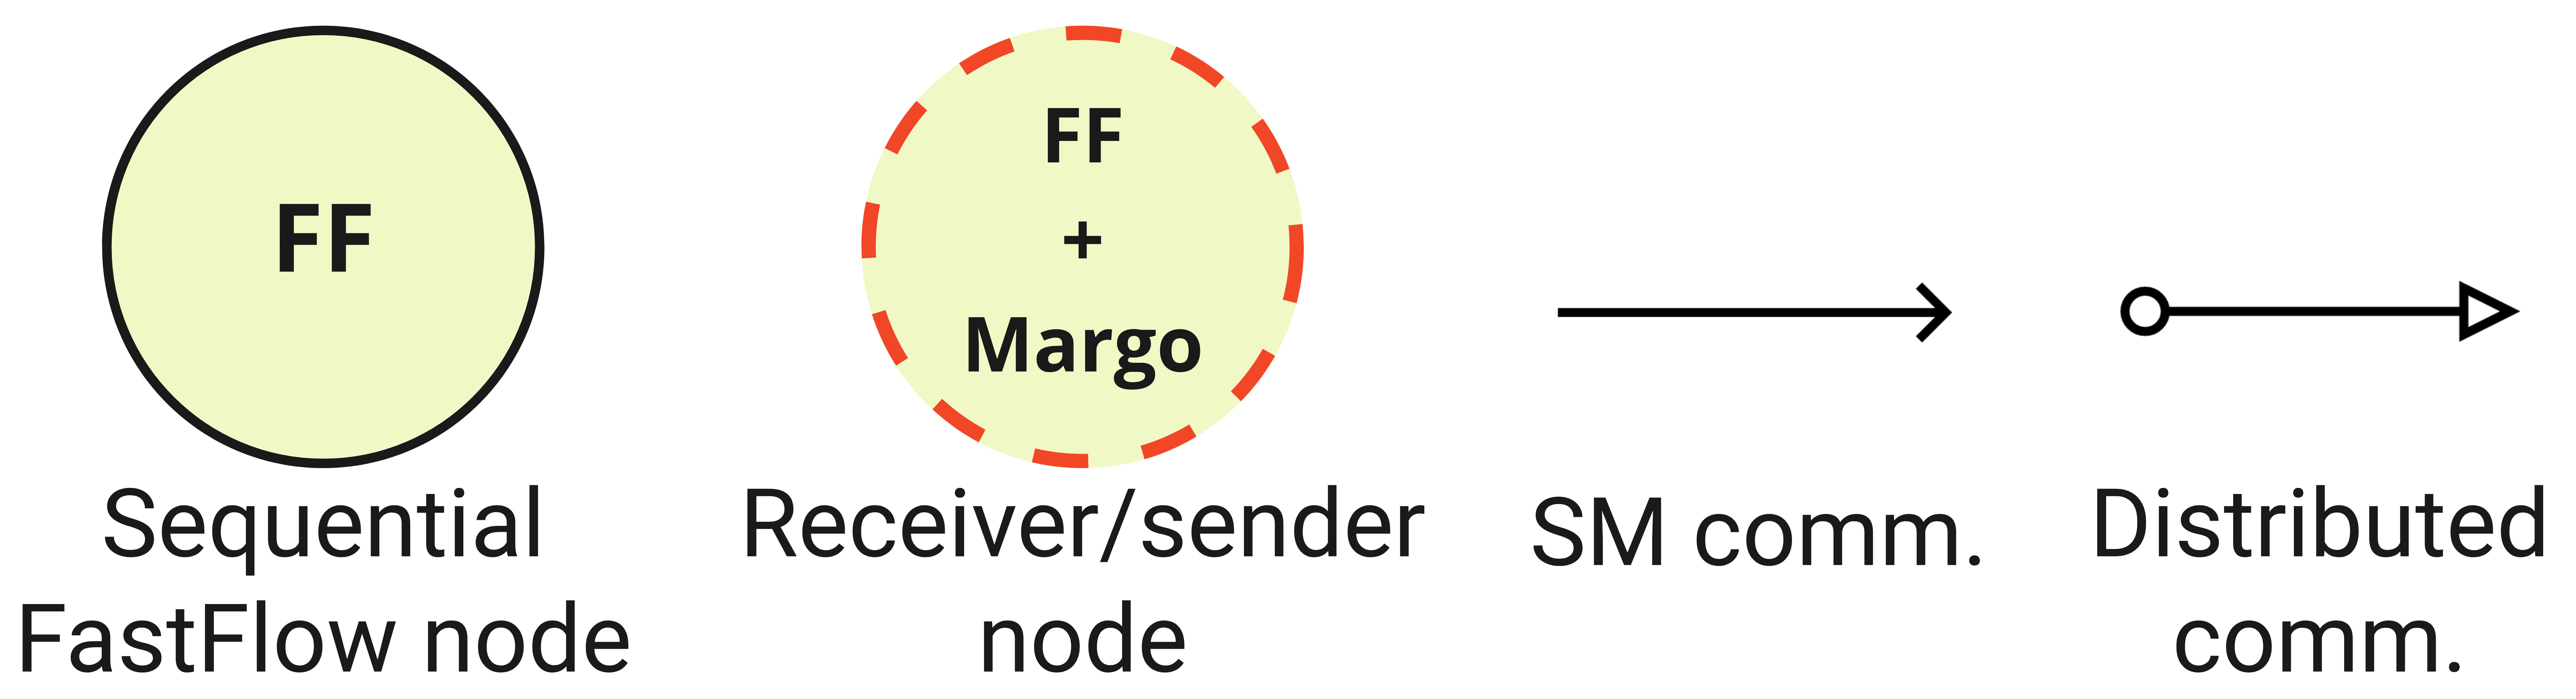
\includegraphics[width=0.6\linewidth]{res/node-legends.jpg}
    \caption{Node legends}
    \label{fig:node-legends}
\end{figure}
\begin{figure}[H]
    \centering
    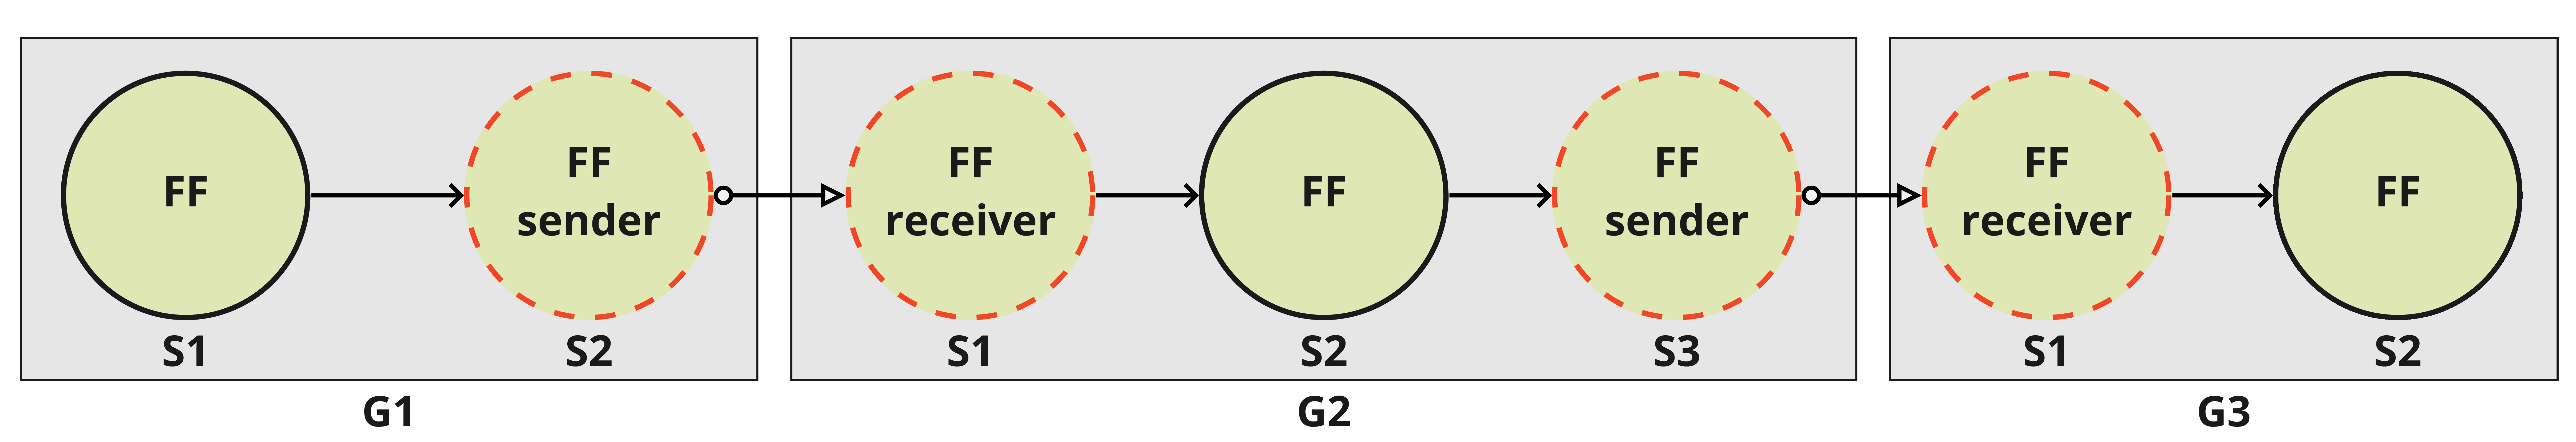
\includegraphics[width=\linewidth]{res/sample-app.jpg}
    \caption{A sample testing application composed of three main groups which are connected by using the implemented classes using Margo library.}
    \label{fig:sample-app}
\end{figure}

Moreover, the standard FastFlow nodes depicted in \hr{fig:sample-app}{Figure} can be any composition of standard FastFlow building blocks. We showed here, for simplicity, a single sequential \ttt{ff\_node\_t}. The important thing to notice is that \ttt{sender} and \ttt{receiver} nodes are mandatory, respectively as last and first nodes, in order to compose distributed groups correctly. The depicted groups represents, potentially, the three situations that may occur when splitting a standard FastFlow application in a distributed one, that are:
\begin{itemize}
    \item (G1): group with only out remote connections. In this case only a \ttt{senderStage} is needed as a last node in the application pipeline. The pipeline is most likely to generate elements from an endo/eso-stream;
    \item (G2): group with both in/out remote connections. Both \ttt{receiverStage} and \ttt{senderStage} are needed, respectively as first and last nodes in the pipeline. All internal nodes receive and send stream elements using Margo-injected nodes;
    \item (G3): group with only in remote connections. Only a first \ttt{receiverStage} pipeline node needed.
\end{itemize}

In \hr{FFMargo-skeleton}{Listings}, we show a skeleton with required library calls necessary to initialize Margo and Argobots environment, which are necessary steps before composing FastFlow building blocks with the implemented communication nodes.

\begin{lstlisting}[language=C++, style=mystyle, caption={Skeleton of a sample FastFlow application using Margo as communication layer.}, label={FFMargo-skeleton}]{FFMargo-skeleton}
int main(int argc, char** argv)
{
    ...

    // Setting up main Argobots instance
    margo_set_environment(NULL);
    ABT_init(0, NULL);

    {
        // Here we place code to build each of the groups composing
        // the application, namely G1, G2, G3.
    }

    // Finalizing Argobots
    ABT_finalize();
}
\end{lstlisting}

After having initialized the environment with the required library calls, we proceed by building the groups that have to be executed as follows:
\begin{itemize}
    \item group G1: implemented in \hyperref[G1-node]{\textbf{Listing \ref{G1-node}}}, creates two nodes, the first one is a simple FastFlow \texttt{ff\_node\_t} generating a stream of elements to forward to other nodes, the second one is a \texttt{senderStage} initialized with the address of the \texttt{receiverStage} to which elements will be forwarded using the Margo communication mechanisms;
    \item group G2: implemented in \hr{G2-node}{Listing}, builds three stages, where the first and the last one are communicator nodes, respectively a \ttt{receiverStage} and a \ttt{senderStage}. The middle node is a simple \ttt{ff\_node\_t} which simply lets tasks flow between the two nodes communicating with groups G1 and G3;
    \item group G3: implemented in \hr{G3-node}{Listing}, builds a \ttt{receiverStage} and a standard \ttt{ff\_node\_t} node which simply prints the tasks received.
\end{itemize}

\begin{center}
\begin{minipage}{.45\textwidth}
\begin{lstlisting}[caption=G1 node composition,language=C++, style=mystyle, label=G1-node]{G1-code}
firstStage  first(stream_len);
senderStage sender(receiver_addr);
ff_Pipe<float> pipe(first, sender);
if (pipe.run_and_wait_end()<0) {
    error("running pipe");
    return -1;
}
\end{lstlisting}
\end{minipage}\hfill    
\end{center}

\begin{center}
\begin{minipage}{.63\textwidth}
\begin{lstlisting}[caption=G2 node composition,language=C++, style=mystyle, label=G2-node]{G2-code}
// Build addresses vector
...

receiverStage receiver(addresses);
forwardStage first;
senderStage sender(receiver_addr);
ff_Pipe<float> pipe(receiver, first, sender);
if (pipe.run_and_wait_end()<0) {
    error("running pipe");
    return -1;
}
\end{lstlisting}
\end{minipage}
\end{center}

\begin{center}
\begin{minipage}{.63\textwidth}
\begin{lstlisting}[caption=G3 node composition,language=C++, style=mystyle, label=G3-node]{G3-code}
// Build the addresses vector
...

receiverStage receiver(addresses);
forwardStage first;
ff_Pipe<float> pipe(receiver, first);
if (pipe.run_and_wait_end()<0) {
    error("running pipe");
    return -1;
}
\end{lstlisting}
\end{minipage}
\end{center}

With the implemented classes, building various groups communicating between each other is very simple and straightforward. Moreover, the way communications are abstracted by the underlying frameworks, makes it easy and painless to extend functionalities of the communication nodes. Adding new protocols requires zero effort and no code modifications from the user point-of-view, since the only step to follow is to define a Mercury-accepted string with the preferred protocol to use during communication and use it at initialization of the receiver node.\newline

Note that, since the receiver stages can be initialized with a vector of strings which represents all the endpoints to which the receiver will listen on, we can (and we must, to allow correct termination) compose multiple instances of groups (G1) and (G2), based on the amount of endpoints created, respectively by (G2) and (G3). For example, if we create a group (G2) with two listening endpoints, in order to allow the whole application to terminate correctly, we must run two (G1) connecting, in turn, to both the endpoints.